\chapter{Version Control} \label{chapter:version-control}
The previous chapter posed the question whether version control can simplify the content authoring process of e-learning content. Before going on and looking at how this process looks like, this chapter briefly introduces the reader to the concept of version control. A solid understanding of version control, its functionality and the context it is used in, will be necessary in order to follow the argument of this thesis during the subsequent chapters.

In the beginning, version control is properly defined and a summary of its most common features is given. Afterwards, the history of version control is outlined and the most popular version control software is shortly introduced. The last section focuses on Git and Github, being the most widely adopted VCS as of today, and also the one that was used throughout this project.

\section{Definition}
Perhaps, version control is best summarized with the words of Hunt and Thomas: "A source code control system [is] a giant UNDO key–a project-wide time machine" \cite{hunt_pragmatic_1999}. Version control, as it is referred to throughout this thesis, goes by several other names as well, such as source code control, revision control or source code management. Nevertheless, these different terms all refer to more or less the same thing: a system that keeps track of changes made to a set of files in a particular location, usually called repository \cite{ruparelia_history_2010}. A new version of a document can be added by \textit{committing} to the repository. This action creates a unique version number and associates author, time and a short description with the state of the content. This allows users to reverse changes and retrieve a particular version of a file from the past. Furthermore, version control simplifies collaboration by offering automated merging of distinct changes made to the same file. For these reasons, and because it works well with text-based documents and source code in particular, version control is used heavily within the software development community \cite{_stack_2015}.

%Most version control systems have additional features, such as automated \textit{merging} of files as well as \textit{branching}, which allows keeping several parallel versions of a project.
%enables its users to keep different versions of a document. The system records changes that are made to a document, thus allowing users to go back in time and recover older versions. Furthermore, it can simplify collaboration through automated merging of files. Thus, when two people have edited the same file and want to bring their changes together, the system offers a way of doing so.
% A VCS enables developers to keep historical versions of source code and project files that are under development and thereafter to retrieve past versions
% the management of changes to document
%  to keep track of different development versions of source code.
% A version control system (also known as a Revision Control System) is a repository of files, often the files for the source code of computer programs, with monitored access.


\section{Taxonomy and Features}
The features described below are mostly shared between different version control systems. Nevertheless, no system is like the other and the naming can vary somewhat from software to software. For this reason, Git, the most widely adopted version control software \cite{_stack_2015} was chosen as a basis. The features are explained conceptually, so that the reader will be equipped to follow the reasoning of this thesis. For a more technical and detailed description of the inner workings of version control other sources can be consulted \cite{baudis_current_2009,chacon_pro_2009,pilato_version_2008}.

\begin{figure}
 \centering
 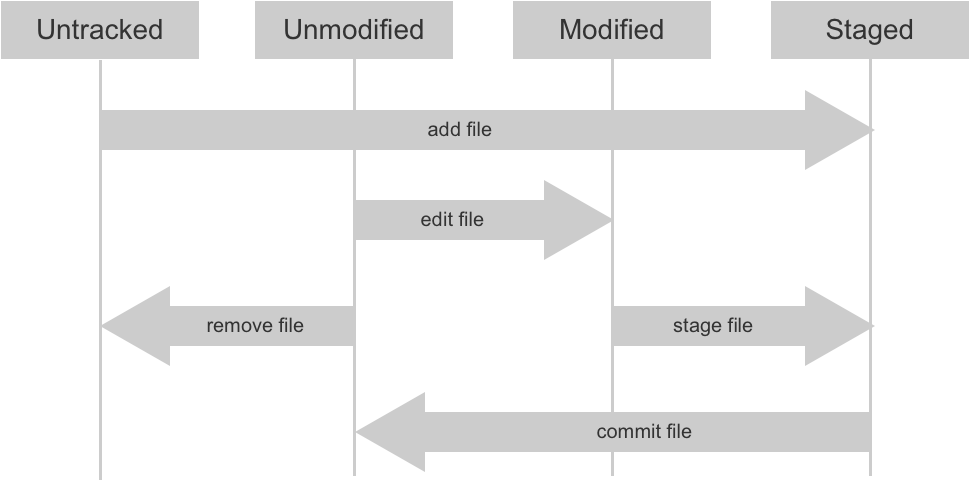
\includegraphics[width=10cm]{version-control/state_of_files}
 \caption{The lifecycle of a file, illustration adapted from Chacon \cite[p.~45]{chacon_pro_2009}.}
 \label{fig:file-state}
\end{figure}

\begin{itemize}
  \item Repository: a database that holds file contents and all versions since creation. A new repository can be created by issuing the \textit{init} command inside a directory. This means that from that moment all files in the directory and its sub-directories can be tracked by version control, unless told otherwise. Repositories can be either local (situated on the client machine) or remote (on the server).
  \item Branching: a branch is a named copy of the entire content stored inside the repository. It allows developers to build features without influencing the stable code. Branches can also be utilized to experiment in case one does not know whether a certain direction will lead to the desired solution.
  \item Tracked, untracked and ignored files: when a new repository is created it is empty. It has to be specifically told which files from the working directory should be tracked. This can be done by using the \textit{add} and \textit{commit} commands. The add command can be used for tracking formerly untracked files and for adding changed files to the staging area (see Figure \ref{fig:file-state}). Once a file is added to the version control system it is in one of three different states: unmodified, modified and staged (ready for committing). If certain files should not be tracked, they can also be ignored permanently.
  \item Working directory: the working directory is the directory which files are tracked  by the version control system. It represents the current state of the files based on the last commit plus the changes that were done since then. It always represents the state of the currently selected branch, which means that the contents of the directory might change based on which branch is selected. The directory can additionally include untracked or ignored files.
  \item Staging area: this is a layer in between working directory and repository. It allows developers to control in a fine-grained way what exactly will be part of the next commit.
  \item Snapshotting: the process of adding a new version to the history of the repository is called snapshotting. It involves adding changes to the staging area (using the add command) and committing these together with a description of what has changed.  Before staging one can also check what has changed compared to the previous version using the \textit{diff} command. The different states a file can be in during its lifecycle are visualized in Figure \ref{fig:file-state}.
  \item Merging: the opposite of branching, merging brings different versions of the same file back together. Usually this is automated, but sometimes conflicts occur, when both versions have changes in the same line of code.
  \item Pull Request: a pull request is a formalized way of letting collaborators review changes that are part of a particular branch before these changes are merged into another branch (usually the main branch). The feature enforces the best practice of \textit{peer reviews} and simplifies the communication between developers. It is not part of Git itself but was introduced by Github (Figure \ref{fig:github-pr}).
\end{itemize}

Figure \ref{fig:git-workflow} provides an overview of a typical Git workflow. The cycle always starts with branching off the main development line and ends in merging back into it. In between the developer writes code and commits this code in coherent pieces, so that reviewing is made easier for collaborators. The pull request is just a way of formally asking these collaborators to review a particular chunk of code. It is a Github feature and not part of Git itself.

%write about reviewing changes (by other developers)

\begin{figure}[h]
 \centering
 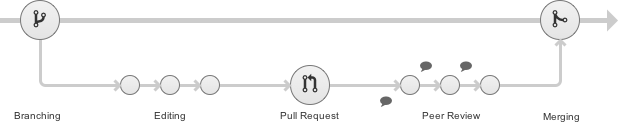
\includegraphics[width=\textwidth]{version-control/git_flow}
 \caption{A common version control workflow, illustration adapted from Github guides \cite{_understanding_????}.}
 \label{fig:git-workflow}
\end{figure}


\section{Version Control Software}
The concept of version control is older than some people might think. Early implementations, such as SCCS (Source Code Control System) or RCS (Revision Control System) date back to the 1970s and 80s \cite{rochkind_source_1975}. According to Sink \cite{sink_version_2011} version control software evolved in three stages: first generation systems only allowed editing one file at a time that had to be locked while changing it. Second generation systems introduced networking and a central repository for simplifying collaboration. Additionally, the concurrent editing of files was now possible. Apache Subversion, still the second-most popular VCS as of 2015 \cite{_stack_2015}, belongs to this generation. The third generation of version control systems were distributed (instead of centralized), no longer file-based and made branching more convenient. Distributed systems are faster, because the network latency for talking to a central repository is eliminated. Furthermore, third generation systems handle large code-bases more efficiently because these systems do not store copies of each file, but only the changesets. This also makes branching a lot quicker and easier. The most widely used VCS among these third generation systems is Git, which is also described in more detail below.

\section{Git and Github}
Git is an open-source version control software that has its origins in the Linux kernel developer community. After running into licensing issues with a proprietary version control software called BitKeeper, the community developed Git in 2005 in order to replace it \cite{chacon_pro_2009, ruparelia_history_2010}. The design of Git was based on BitKeeper and the requirements of the Linux developer community. Because it is distributed and changes do not need to be committed to a central repository it is faster than most other VCSs. Furthermore, it supports hundreds of parallel branches and handles large code bases like the Linux kernel efficiently. Git is also workflow agnostic. There is no access management or locking of files. Everyone can edit anything at any time. Conflicts, in case they emerge, are dealt with after the fact, when files are merged together again. As Linus Torvalds said in a presentation in 2007, Git is based on "a network of trust"\footnote{https://www.youtube.com/watch?v=4XpnKHJAok8}. Companies can decide for themselves what kind of rules or workflows they want to enforce. These characteristics have made Git the most popular VCS in software development by far, beating Subversion as a distant second (69\% vs. 37\% adoption) \cite{_stack_2015}.

\begin{figure}[h!]
 \centering
 \fbox{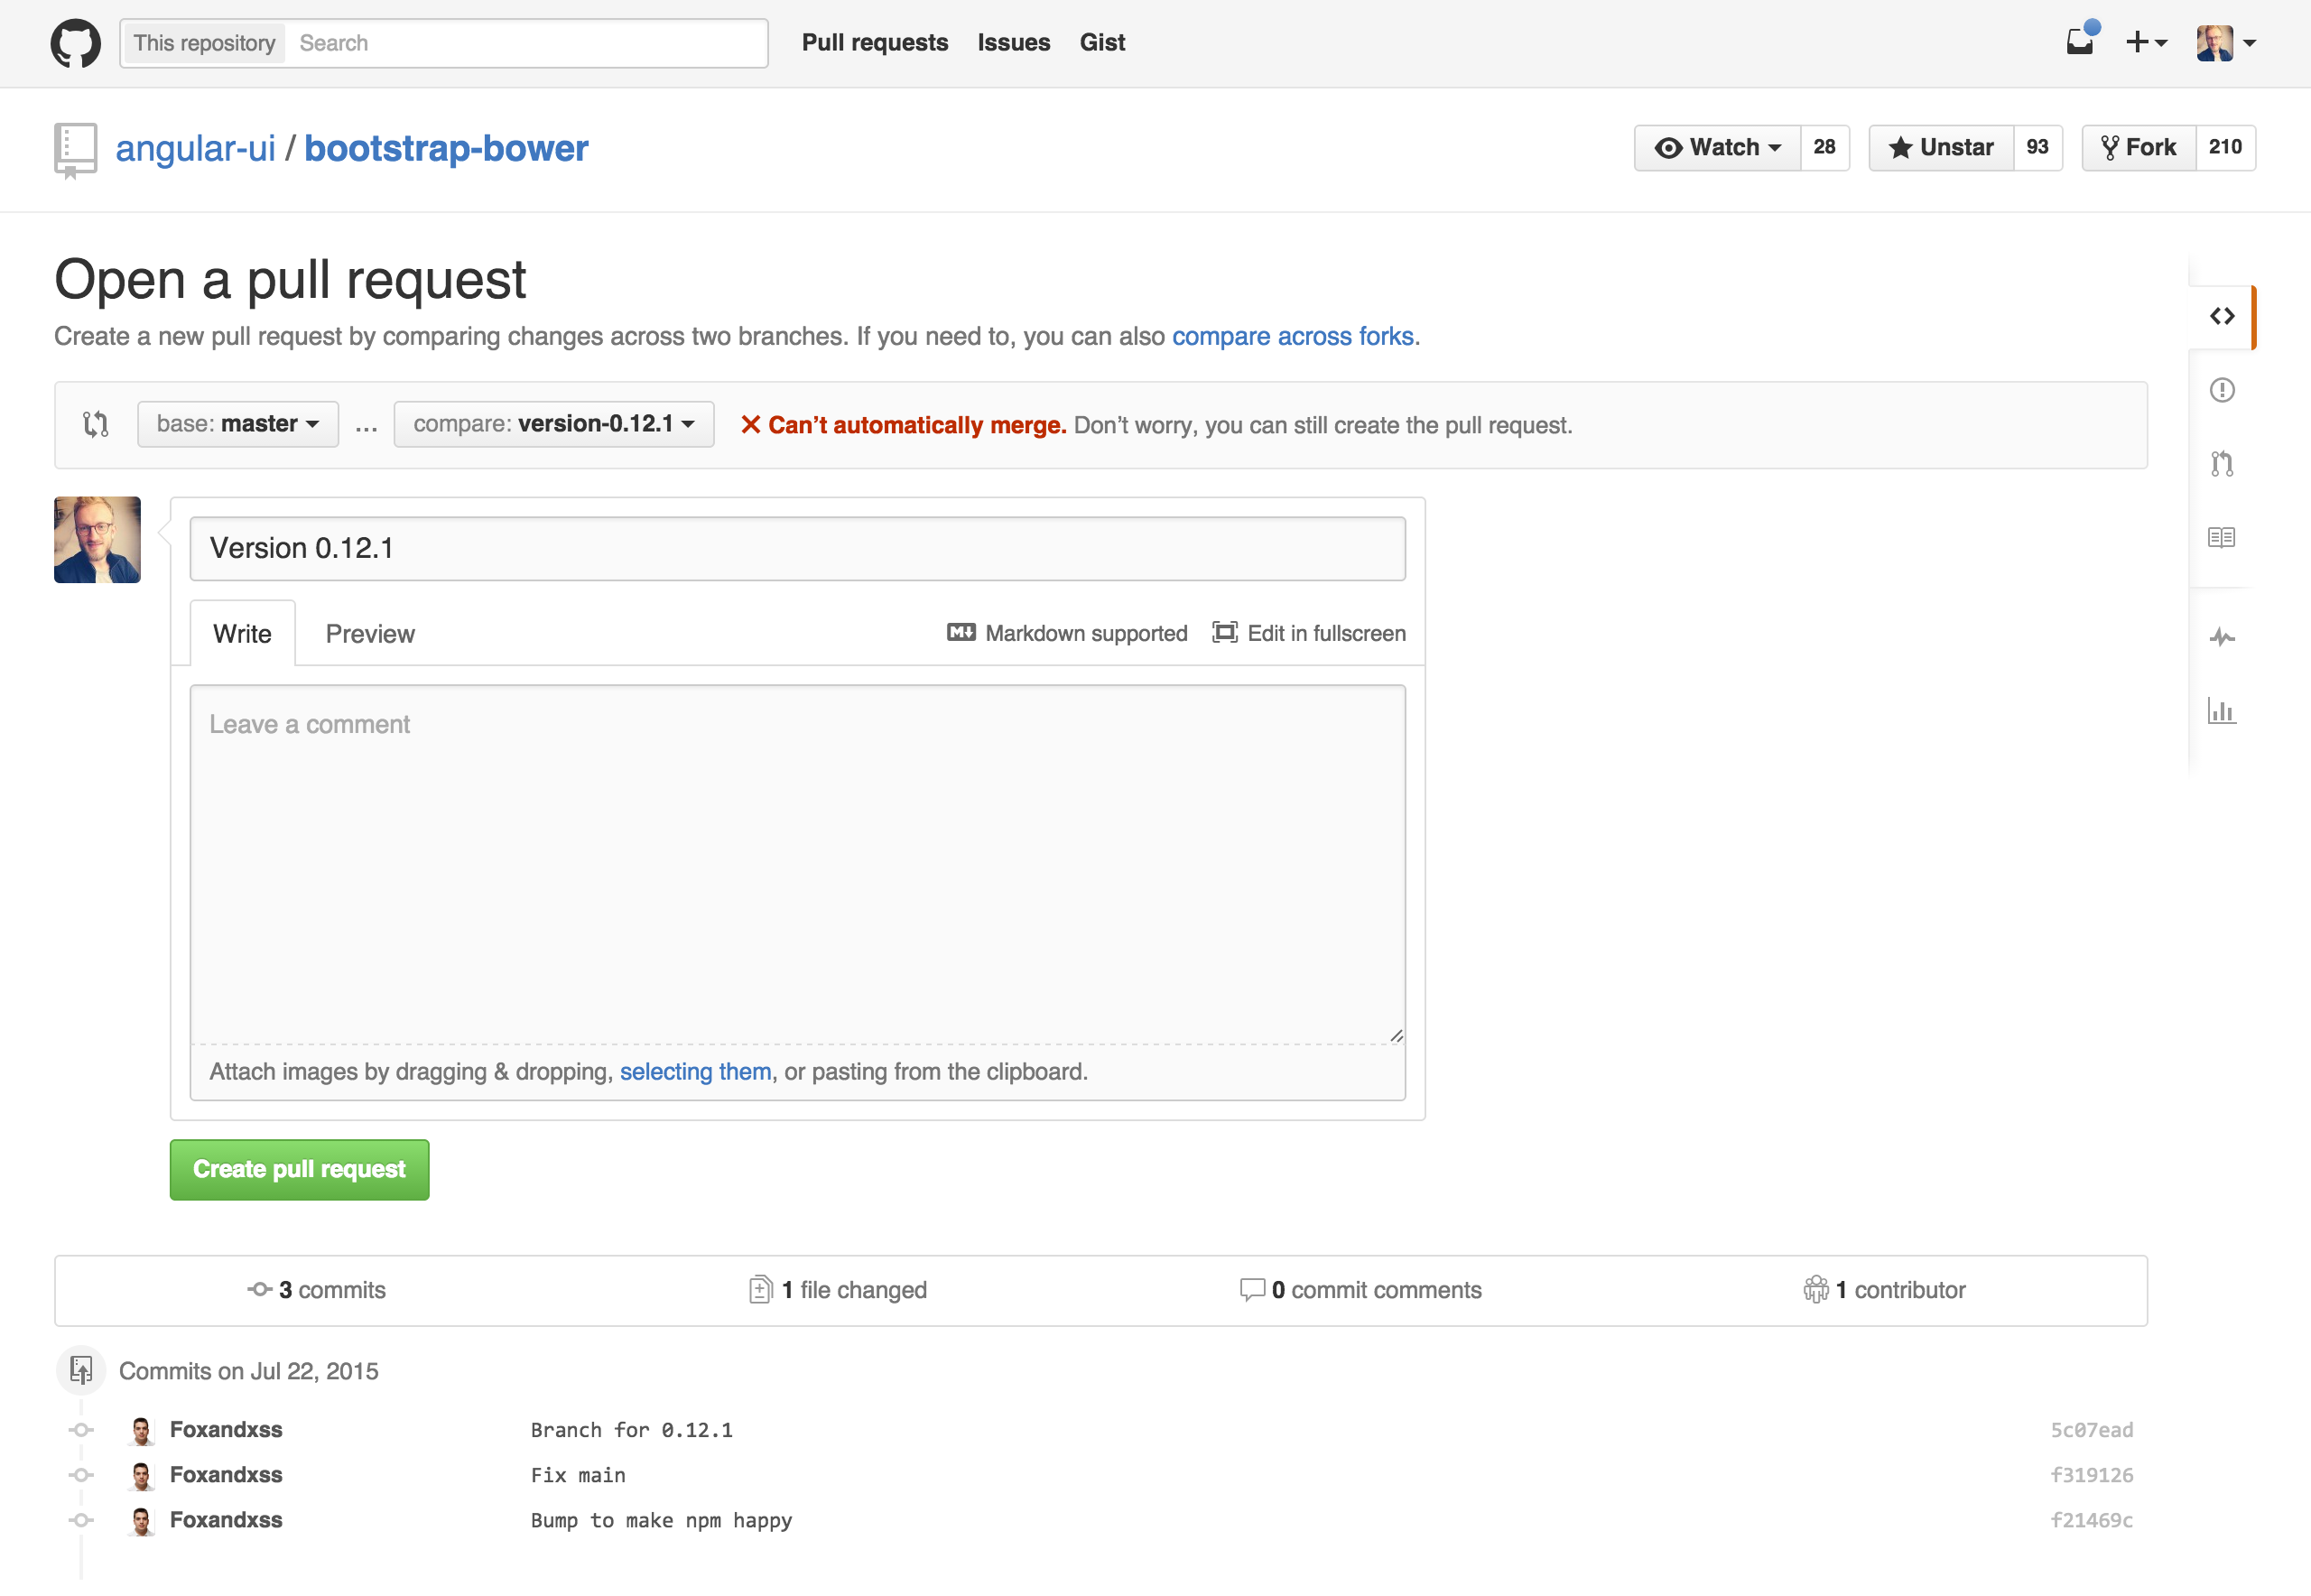
\includegraphics[width=12cm]{version-control/github-pull-request}}
 \caption{Pull request view on Github}
 \label{fig:github-pr}
\end{figure}

Github, like the name gives away, is based on Git. It is a repository hosting service that adds additional features, such as access control and social networking capabilities\footnote{http://techcrunch.com/2012/07/14/what-exactly-is-github-anyway/}. The service eliminates the need of setting up a personal server in order to host a  repository and makes collaboration simpler by offering wikis, task management and a mechanism for code reviews. All of this is offered through an easy to use graphical user interface. Furthermore, it has become the de-facto standard for sharing open-source projects.

\section{Conclusion}
Version control software is used to keep track of changing code-bases and for simplifying collaboration among developers. Even though some VCSs have been around for a few decades, the widespread adoption of version control has started only with the second generation of version control systems. Distributed VCSs as well as cloud services, such as Github, have further accelerated this adoption.

Now that the concept of version control might be a little clearer, the next chapter will look at research that investigated the usability of different version control systems. Furthermore, several projects are described which employed version control outside of its "natural habitat" of software development.

% version control is used by a large majority of programmers
% git is the most popular, subversion is second

%\section{Advantages and Disadvantages}
%A version control system allows a developer to keep track of every change that has been made to a source code as well as reversing changes that broke the code. Strangely enough this approach has not made its appearance in a lot of other areas yet. Although Google Docs features a revision history \cite{_google_2010} \cite{30_google_????}, most other software still utilizes simpler means of error-avoidance such as prompts (“Do you really want to delete this file?”) or simple undo actions through the ctrl-z-command. But for systems that handle a lot of data these approaches are very limited and sooner or later users will run into problems (How do I get back to something I changed yesterday?).

%Another reason why developers use version control systems is the simplified collaboration with other developers \cite{spinellis_version_2005}. Before version control, a developer could only edit a piece of code if he or she was sure that no one else was working on it at the same time. Otherwise it would have been nearly impossible to combine the changes that were made by different developers. Most version control systems release the developer from the burden of thinking about this aspect of his or her work. Either through a mechanism called \textit{file locking}, through which the system ensures that only one developer at a time can edit a file, or through something called \textit{automatic merging} \cite{pilato_version_2008}. A functionality that allows changes that were made in the same file to be automatically combined in case there are no overlaps (changes in the same line of the file). This permissive approach usually works well, because even when two developers are working on the same file, they rarely modify the same procedure or module.

%A third advantage of version control, besides easy reversibility and collaboration, is the higher accountability of contributors. Currently, Babbel gives full access to everyone who has the slightest need of accessing the content. This not only includes members of the didactics team, but also people responsible for technical quality assurance or marketing. Everyone can, in theory, manipulate data that effects the live system the end user is exposed to. Because of the suboptimal usability of the system, errors can be introduced accidentally or data can be modified that should not be modified. A version control system makes these changes visible and allows to identify individuals who made changes they were not supposed to do. Currently an employee might never learn that he or she did something wrong.
